% LaTeX .tex
% Example for the proceedings of the  25th International Congress of Mechanical Engineering
% COBEM 2019
% October, 20-25, 2019, Uberlândia, MG, Brazil
% Based on the template of the proceedings of COBEM2015 and COBEM2017

\documentclass[10pt,fleqn,a4paper,twoside]{article}
\usepackage{abcm}
\def\shortauthor{V. Obadowski, T. Batista and P. Miyagi}
\def\shorttitle{Modeling of Naval Propulsion -- Approach Based on Hybrid Systems}

\begin{document}
	\fphead
	\hspace*{-2.5mm}\begin{tabular}{||p{\textwidth}}
		\begin{center}
			\vspace{-4mm}
			\title{MODELING OF NAVAL PROPULSION -- APPROACH BASED ON HYBRID SYSTEMS}
		\end{center}
		\authors{Vinícius Novicki Obadowski} \\
		\authors{Thalles Andrade Estrela Batista} \\
		\authors{Paulo Eigi Miyagi} \\
		\institution{Escola Politécnica da Universidade de São Paulo} \\
		\institution{obadowski@usp.br, thalles.batista@usp.br and pemiyagi@usp.br} \\
		\\
		\abstract{\textbf{Abstract.} This paper proposes a model for a full electric naval propulsion system using object-oriented differential predicate transition Petri nets (OO-DPT). This approach encompasses discrete events characteristics as well as the continuous values. To formulate this model, it was adopted the Production Flow Schema methodology in order to describe the system behavior and its main components and equipment. And after, using OO-DPT Petri Nets, a hybrid systems approach, it is possible to build a comprehensive model.}\\
		\\
		\keywords{\textbf{Keywords:} naval propulsion, hybrid systems, Petri Nets, Objected-oriented Differential Predicate Transition Petri Nets, submarine}\\
	\end{tabular}
	
	\section{INTRODUCTION}
	\label{sec:intro}
	
	% Basic information about submarine design and motivation on Brazil
	There has been an effort of brazilian government in developing technologies related to naval projects in the last years, especially because of some military driven projects such as PROSUB ({\it Programa de Desenvolvimento de Submarinos})~\citep{Brasil2013}. This government program aims to obtain submarines as well as design technologies for them, in this way enhancing the independence of Brazil regarding this specific type of technology.
	
	% Complexity linked to submarine design
	However, development of naval projects -- especially those related to submarines -- is a complex and a time consuming task, often involving an engineering team with many professionals that have different skills and expertise. Some authors reckon that military submarines can be treated as complex projects \citep{Chalfant2015} \citep{Cooper2017}, given these often include several knowledge areas, such as: electrical, mechanical, marine, control and automation engineering to design each part of a submarine.
	
	% Collaborative submarine design
	Consequently, to be able to design a submarine, engineers should work in cooperation, discussing the project among themselves and coordinating their future steps, to ensure that the submarine design is being done with consistency. Regarding this kind of approach, \citet{Langland2015} describes how to address this matter over a multidisciplinary environment, where different disciplines are thought together in order to achieve results that fulfill clients requirements. This approach relies on building models for each discipline at same multiple requirements from other areas are evaluated \citet{Chalfant2017b}.
	
	% Simulation modelling
	Building a mathematical model of a system for simulation, it allows one to verify and to analyze behaviors, values and make decisions based on results obtained \citep{Chung2004}. Considering, that submarine design involves a lot of people and requires project consistency, develop a model for it is a condition necessary to verify premises adopted as well as to ensure that expected performances are being achieved.
	
	% Hybrid systems
	Nevertheless, before building a model, the developers must observe which are their goals and parts that are going to be modelled. In case of submarine design at early stage, the design team is looking for translate client requirements into a feasible submarine. To achieve this, they should estimate values of submarine' size and weight, thermal and electrical needs and several other subjects \citet{Pereira2016}.
	
	% Naval Propulsion and Hybrid Propulsion
	Taking into account the Brazilian Navy objectives, development of models for submarine components can improve design approaches and can aid during verification of the project itself. This is particularly relevant for propulsion and electrical systems, given they are responsible -- in a conventional submarine -- for power generation, for power storage and for propelling the submarine~\citet{Pereira2016}. However, a traditional approach of continuous variables will not encompass all behavior of these two systems, because their operation relies on human commands that made decisions based on external actors or events. Similarly, using a model that uses only discrete events will not address the systems properly, as continuous variables may trigger events. Therefore, an approach that deals with both continuous variable and discrete events is required, hence a hybrid system approach can be used to model these systems.
	
	% Catch for the paper part
	In this paper, it is discussed a model for a conventional submarine based on hybrid systems, considering its expected operation and performances. The main goal is to build a model that represent these and can be used by a design team to improve its project. In the following sections, a short review of naval propulsion is presented, as well as details regarding the methodology chosen, the model described in Production Flow Schema (PFS) and results.
	
	\section{NAVAL PROPULSION DESCRIPTION}
	\label{sec:naval}
	% An overview about naval propulsion - full electric, no need to speak about everything that exists in the world. Not now.
	\citet{Geertsma2017} points out that there are several ways to build a naval propulsion system. Such as, using a prime mover directly attached to shaft line, or a electrical propulsion motor (EPM) instead of a prime mover. The power generation can be done by diesel or gas generators or for some small ships using solar panels, the power storage might be performed by traditional lead-acid batteries or fuel cells. The decision of using which combination of technologies are left for designers that take into account client objectives for the ship. A review about different types of naval propulsion and their common application is discussed in \citet{Geertsma2017}.
	
	Accordingly to~\citet{Pereira2016}, for a conventional submarine the usual propulsion adopted is the one known as ``full electric'', because all mechanical power deliver to the submarine's propeller is provided by an EPM, the electrical power is generated by a diesel generator and this energy stored in batteries. Despite existing other types of propulsion arrangements, the ones that combine prime movers along EPM or that employs only prime movers are not usually used in undersea vehicles. Because, they do not operate on an environment with oxygen available, use of systems that rely on fresh air are discarded. Figure~\ref{fig:full}\ depicts an overview from electrical point of view of a ``full-electric'' propulsion system for a conventional submarine, where portside and starboard are represented in red and green colors, respectively.
	
	\begin{figure}[h!]
		\centering
		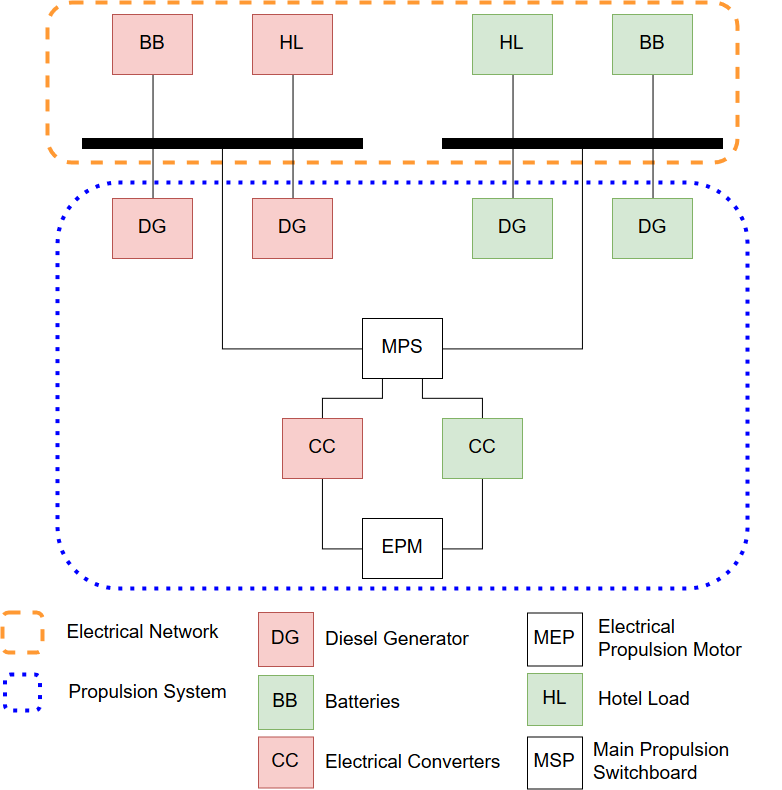
\includegraphics[angle=0, scale=0.400]{prop_arch.png}
		\caption{``Full-electric'' propulsion for a conventional submarine based on works of \citet{Geertsma2017} and \citet{Pereira2016}.}
		\label{fig:full}
	\end{figure}
	
	
	\section{METHODOLOGY}
	\label{sec:method}
	
	% Describe overview of Villani methodology
	% There is a chapter in thesis that present the topic
	% Cover: what are hybrid system (small background) and the methodology (in bullets of course)
	
	Considering that submarines are complex systems as explained in section~\ref{sec:intro}\ , \citet{Villani2004}
	
	\begin{enumerate}
		\item Modelling the flows of material
		\item Specification of the use cases
		\item Building the activity diagrams
		\item Specification of classes and objects
		\item Building the sequence and collaboration diagrams
		\item Building the OO-DPT net of the classes and the class diagrams
		\item Verification of consistency between models
	\end{enumerate}
	
	\section{MODEL}
	\label{sec:model}
	% Well, the model, essencially the first step PFS. The further steps shall be presented in the complete article, that will encompass all other steps given by Villani's methodology.
	The Production Flow Schema (PFS) presented by \citet{Miyagi1996}\space
	
	Based on description provided by in section~\ref{sec:naval}\space, it is possible to start to model a naval propulsion
	
	% %ACKNOWLEDGEMENTS section
	% \section{ACKNOWLEDGEMENTS}
	% \label{sec:ack}
	%
	% This study is supported by Brazilian Navy.
	
	\bibliographystyle{abcm}
	\renewcommand{\refname}{}
	\bibliography{library}
	
	\section{RESPONSIBILITY NOTICE}
	\label{sec:legal}
	
	% No need for changes here.
	The authors are the only responsible for the printed material included in this paper.
	
\end{document}
